\documentclass{article}
\usepackage{amsmath}
\usepackage{graphicx}
\usepackage{xepersian}

% set font
\settextfont{B-NAZANIN.ttf}[
	Path = fonts/ ]
\setlatintextfont{Vazir.ttf}[
	BoldFont = Vazir.ttf, 
Path = fonts/ ]

\title{ شبکه های عصبی و یادگیری عمیق}
\author{تهمینه توکلی}
\date{تیر ۱۴۰۳}

\begin{document}

\maketitle

\section{مقدمه}
در این پروژه، رویکرد جدیدی برای بهبود عملکرد طبقه بندها با استفاده از ایده‌های دو مقاله تاثیرگذار بررسی می‌شود: "یک روش یادگیری ویژگی تفکیکی برای تشخیص چهره عمیق" و "دشمن دشمن من دوست من است: بررسی دشمنان معکوس برای بهبود آموزش مقاومتی". هدف اصلی، بررسی این است که آیا می‌توان از دشمنان معکوس به جای مراکز داده ها در تابع زیان استفاده کرد تا قدرت تفکیکی مدل‌های طبقه بند را افزایش داد.

\section{پیش‌زمینه}
\subsection{تشخیص چهره عمیق با استفاده از \lr{center loss}}
مقاله "یک روش یادگیری ویژگی تفکیکی برای تشخیص چهره عمیق" \lr{center loss} را معرفی می‌کند که هدف آن افزایش قدرت تفکیکی ویژگی‌های یاد گرفته شده توسط شبکه‌های عصبی عمیق است. این تابع زیان فاصله بین ویژگی‌های یک کلاس و مرکز آن کلاس  در فضای ویژگی‌ها را کاهش می‌دهد. منظور از فضای ویژگی‌ها، خروجی لایه ماقبل آخر مدل است که توسط
\lr{feature extractor}
یاد گرفته شده است. این کاهش واریانس درون کلاسی به بهبود استحکام و دقت مدل کمک می‌کند.

\begin{figure}[h]
    \centering
    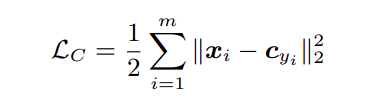
\includegraphics[width=0.4\textwidth]{cl-formula.png}
    \label{fig:sample_figure}
\end{figure}

در معادله ۱،
$x_i$
نشان دهنده ویژگی $i$م و متعلق به کلاس
$y_i$
است
و
$c_{y_i}$
مرکز کلاس
$y_i$
در فضای ویژگی‌ها را نشان میدهد. مرکزها در طول یادگیری به روزرسانی می‌شوند.

\begin{figure}[h]
    \centering
    \begin{minipage}[b]{0.45\textwidth}
        \centering
        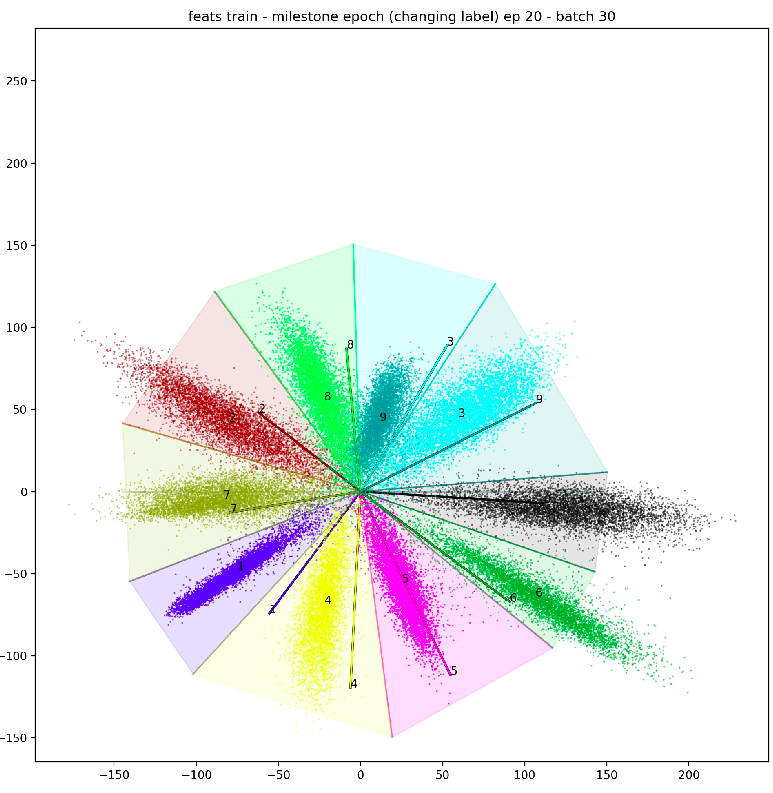
\includegraphics[width=\textwidth]{ce.png}
    \end{minipage}
    \hfill
    \begin{minipage}[b]{0.45\textwidth}
        \centering
        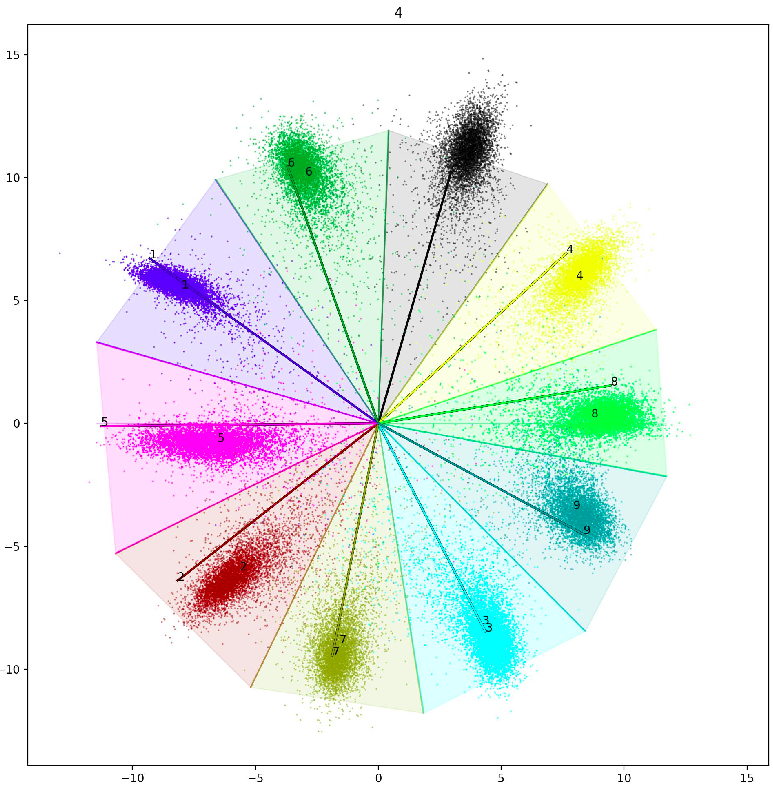
\includegraphics[width=\textwidth]{cl.png}
    \end{minipage}
    \caption{
    توزیع ویژگی های آموخته شده تحت نظارت \lr{cross entorpy loss} (سمت راست) و \lr{center loss} (سمت چپ). نقاط با رنگ های مختلف نشان دهنده ویژگی ها از کلاس های مختلف است. بردار وزن هر کلاس و میانگین ویژگی های هر کلاس مشخص شده است.
    }
    \label{fig:sample-images}
\end{figure}

شکل ۱ مربوط به دو مدل تعلیم شده تحت نظارت \lr{cross entorpy loss} (سمت راست) و \lr{center loss} (سمت چپ) است.
با مقایسه دو تصویر در شکل ۲، متوجه میشویم که در صورتی که فقط از تابع زیان 
 \lr{cross entorpy}
 استفاده کنیم، ویژگی‌های عمیق آموخته شده توسط
 \lr{feature extractor}
دارای واریانس درون کلاسی بزرگی خواهند بود.
همچنین برای هر کلاس بردار وزن الزاما با میانگین ویژگی های آن کلاس منطبق نیست.

در صورتی که ویژگی استخراج شده توسط مدل برای یک داده ورودی، دقیقا در امتداد بردار وزن کلاس مربوطه قرار بگیرد، خروجی احتمالی مدل برای این کلاس بیشترین مقدار خواهد بود و داده با اطمینان بالا به درستی طبقه بندی میشود.
در واقع، امتداد بردار وزن هر کلاس نشان دهنده مناطقی است که با احتمال زیاد متعلق به همان کلاس طبقه بندی می‌شوند (\lr {high likelihood regions}).

با افزودن جمله \lr{center loss} به تابع زیان، مشکل واریانس درون کلاسی تا حد خوبی برطرف شده است (تصویر سمت چپ).
اما همچنان قابل مشاهده است که محل قرارگیری میانگین ویژگی های هرکلاس با بردار وزن مربوطه فاصله دارد.
این مشکل در ابعاد بالاتر شدیدتر خواهد بود.

استخراج ویژگی دقیقا در امتداد بردار وزن لزوما برای \lr{feature extractor} قابل انجام نیست.
هدف این پروژه بررسی این است که \lr {high likelihood regions}
در ابعاد بالاتر در چه مکانی قرار دارند به صورتی که برای 
\lr{feature extractor}
تولید ویژگی در این مکان قابل انجام باشد.
آیا \lr {high likelihood regions}
در مکان بردار وزن است یا میانگین ویژگی ها و یا مکانی دیگر؟

\subsection{\lr{Inverse adversarial examples} برای آموزش مقاومتی}
مقاله "دشمن دشمن من دوست من است: بررسی دشمنان معکوس برای بهبود آموزش مقاومتی"، مفهوم \lr{inverse adversarial examples} را معرفی می‌کند که هدف آن افزایش قدرت تفکیک مدل است.
این تابع زیان فاصله بین ویژگی‌های یک کلاس و نمونه های \lr{inverse adversarial} را کاهش می‌دهد.

 این نمونه ها با استفاده از روش نزول گرادیان پیش‌بینی شده (\lr{PGD}) اصلاح شده ساخته می‌شوند که همان معادله \lr{PGD}
است با این تفاوت که در جهت مینیمم شدن تابع زیان حرکت می‌کند.

این نمونه ها در \lr {high likelihood regions}
قرار دارند و با توجه به اینکه روش تولید آنها گرادیانی است، قدرت \lr{feature extractor}
برای استخراج ویژگی در این فضا درنظر گرفته شده است.
بنابرین دشمنان معکوس ممکن است به عنوان مثال‌هایی معنی‌دارتر برای بهبود آموزش مدل عمل کنند.

\begin{figure}[h]
    \centering
    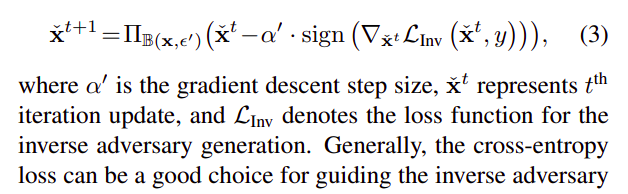
\includegraphics[width=0.7\textwidth]{pgd.png}
    \label{fig:sample_figure}
\end{figure}

\section{هدف}
هدف اصلی این پروژه بررسی این است که آیا نمونه های \lr{inverse adversarial} می‌توانند جایگزین بهتری برای مراکز کلاسی در \lr{center loss} باشند؟
زیرا با توجه به اینکه نمونه های \lr{inverse adversarial} با در نظر گرفتن قدرت \lr{feature extractor} در تولید ویژگی ساخته می‌شوند، احتمالا نزدیک کردن ویژگی ها به این مراکز برای مدل راحت تر است.

برای انجام تحلیل های لازم، دو مدل با تابع زیان عادی و \lr{center loss} تعلیم داده شده اند و سپس نمونه های \lr{inverse adversarial} برای هر مدل تولید شده است. میانگین این نمونه ها برای هر کلاس محاسبه شده است. با توجه به نتایج، فاصله میانگین نمونه های \lr{inverse adversarial} با بردار وزن کلاس ها مقایسه شده است.

\section{روش‌شناسی}
\subsection{آموزش مدل}
برای تمامی آزمایش ها از مدل \lr{TRADES} روی دیتاست \lr{MNIST} استفاده شده است. هر مدل 25 ایپاک با نرخ یادگیری $0.01$ و با روش \lr{SGD} آموزش دیده است.

\begin{enumerate}
    \item \textbf{مدل \lr{A}}: آموزش با \lr{cross entropy}
    \item \textbf{مدل \lr{B}}:  آموزش با \lr{center loss}
\end{enumerate}

\subsection{تولید \lr{inverse adversarial examples}}
با استفاده از مدل‌های آموزش دیده، \lr{inverse adversarial examples} از طریق روش \lr{PGD} اصلاح شده تولید شده اند.
با توجه به پارامترها در مقاله اصلی، این روش با تعداد حلقه تکرار ۲۰ و \lr{step size} برابر $0.01$ و برای مقادیر مختلف پارامتر $\epsilon$ انجام شده است.

\subsection{معیارهای مقایسه فاصله}
مقایسه فاصله مراکز ویژگی‌ها با استفاده از دو معیار انجام می‌شود:
\begin{enumerate}
    \item \textbf{شباهت کسینوسی}: کسینوس زاویه بین دو بردار را اندازه‌گیری می‌کند و شباهت جهت‌گیری بین بردارهای ویژگی را نشان می‌دهد.
    \item \textbf{میانگین مربعات خطا (\lr{MSE})}: میانگین تفاوت‌های مربعی بین عناصر متناظر دو بردار را اندازه‌گیری می‌کند و تفاوت مطلق در بزرگی را نشان می‌دهد.
\end{enumerate}

\section{آزمایش‌ها و نتایج}
همه مدل ها با موفقیت همگرا شدند.
ویژگی‌های استخراج شده از داده های ورودی برای محاسبه مراکز زیر استفاده شدند. برای هر کلاس، میانگین نمونه های \lr{inverse adversarial} (مراکز تخاصمی) با هر سه مورد مقایسه شده است.

\begin{enumerate}
    \item میانگین خود ویژگی‌ها 
    \item مراکز \lr{center loss}
    \item بردار وزن
\end{enumerate}

%%%%%%%%%%%%%%%%%%%%%%%%%%%%%%%%%%%%%%%%%

\begin{figure}[h]
    \centering
    \begin{minipage}[b]{0.45\textwidth}
        \centering
        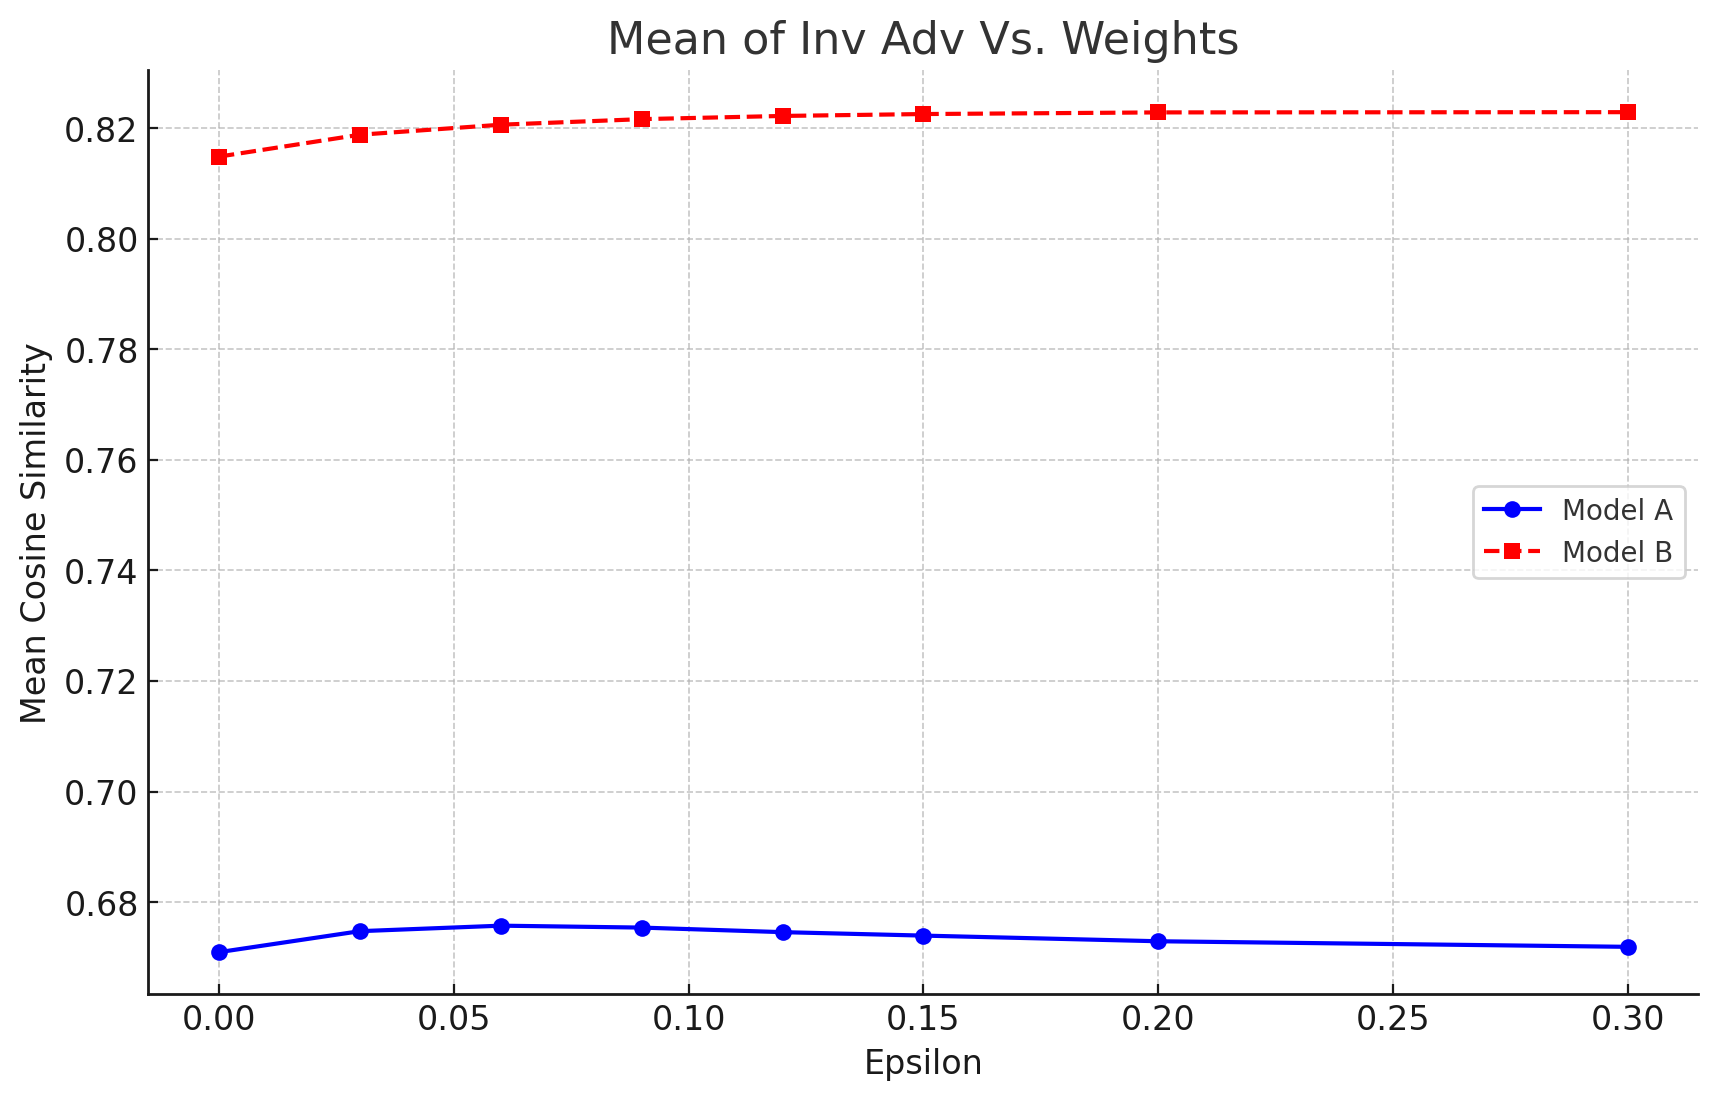
\includegraphics[width=\textwidth]{cl-ce-W.png}
    \end{minipage}
    \hfill
    \begin{minipage}[b]{0.45\textwidth}
        \centering
        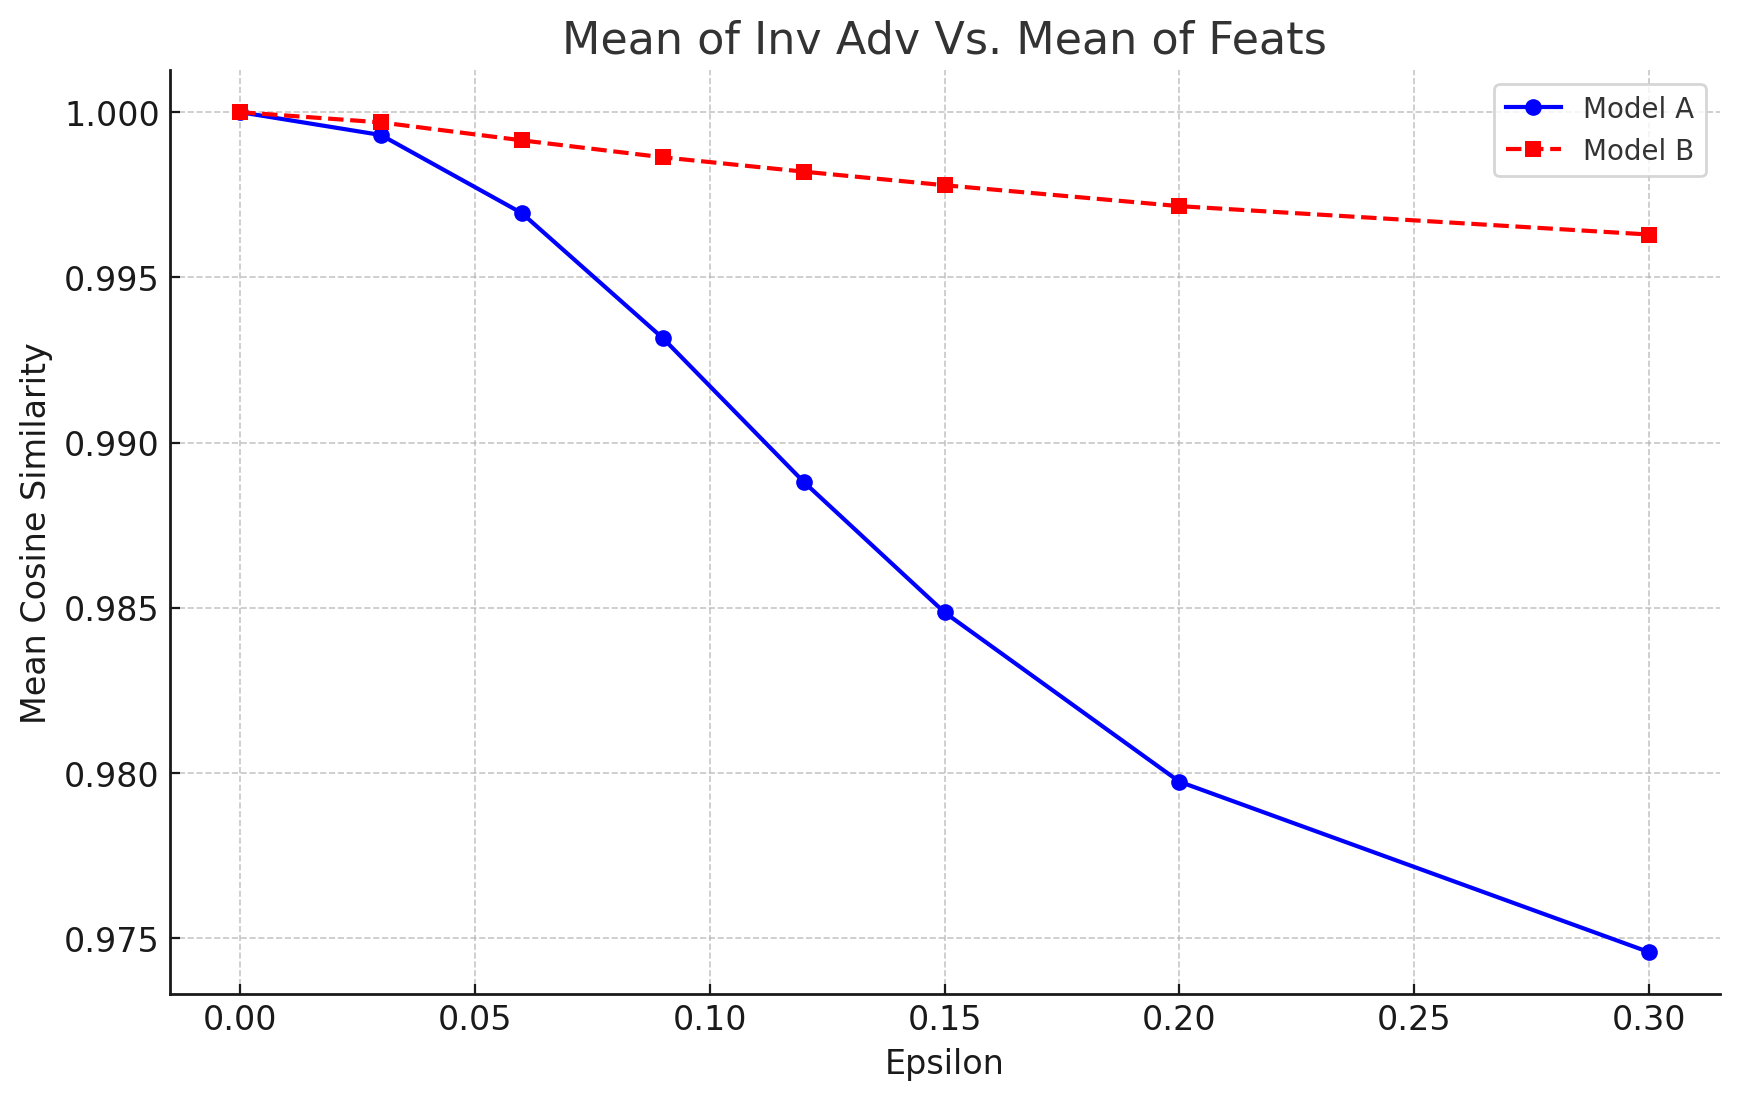
\includegraphics[width=\textwidth]{cl-ce-M.png}
    \end{minipage}
    \caption{
میانگین شباهت کسینوسی بین مراکز تخاصمی و بردار وزن (راست) - مراکز تخاصمی و مراکز ویژگی‌ها (چپ) بر حسب $\epsilon$    
در دو مدل \lr{A} و \lr{B}
    }
    \label{fig:sample-images}
\end{figure}

%%%%%%%%%%%%%%%%%%%%%%%%%%%%%%%%%%%%%%%%%

\begin{figure}[h]
    \centering
    \begin{minipage}[b]{0.45\textwidth}
        \centering
        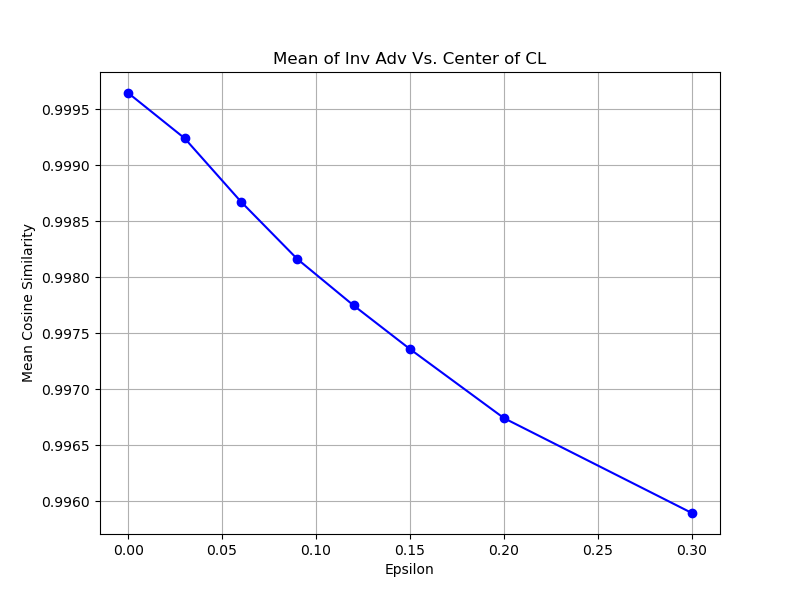
\includegraphics[width=\textwidth]{cl-CL.png}
    \end{minipage}
    \caption{
مدل \lr{B}:  میانگین شباهت کسینوسی بین مراکز تخاصمی و مراکز \lr{center loss} بر حسب $\epsilon$    
    }
    \label{fig:three-images}
\end{figure}

%%%%%%%%%%%%%%%%%%%%%%%%%%%%%%%%%%%%%%%%%

با توجه به شکل ۲ و ۳، افزایش $\epsilon$
باعث کاهش فاصله کسینوسی و در نتیجه افزایش شباهت بین مراکز تخاصمی و میانگین ویژگی‌ها و همچنین افزایش شباهت بین مراکز تخاصمی و مراکز \lr{center loss} (در مدل \lr{B}) می‌شود.

    در مدل \lr{B}، شباهت بالا بین مراکز تخاصمی و مراکز \lr{CL} نشان‌دهنده این است که نمونه های تخاصمی ویژگی‌های جهت‌گیری مراکز سنتی را حفظ می‌کنند.
   شباهت پایین بین مراکز تخاصمی و وزن‌های مدل نشان‌دهنده این است که وزن‌ها به طور مستقیم با مراکز فضای ویژگی‌ها هماهنگ نیستند.

علاوه بر این، شباهت با مراکز ویژگی‌ها در هر دو مدل نشان می‌دهد که نمونه های تخاصمی ویژگی‌های خاص کلاس را حفظ می‌کنند در حالی که واریانس درون کلاسی کاهش نمی‌یابد. تفاوت‌های قابل توجه با وزن‌های مدل تأیید می‌کند که ویژگی‌های فضای ویژگی‌ها با وزن‌های یاد گرفته شده متمایز هستند.


\section{نتیجه‌گیری}
این پروژه نشان می‌دهد که استفاده از \lr{inverse adversarial examples} به عنوان جایگزینی برای مراکز سنتی در \lr{center loss} امکان‌پذیر است.
با توجه به اینکه مراکز تخاصمی شباهت کسینوسی بالا و \lr{MSE} پایین با مراکز سنتی \lr{center loss} دارند، به ویژه در مدل \lr{A}.
این رویکرد نشان می‌دهد که می‌تواند استحکام مدل را افزایش داده و تفکیک‌پذیری و واریانس درون کلاسی ویژگی‌ها را نیز حفظ کند.
تحقیقات بیشتر می‌تواند به بهینه‌سازی تولید \lr{inverse adversarial examples} و یکپارچه‌سازی این رویکرد در چارچوب‌های دیگر یادگیری تفکیکی بپردازد.

\pagebreak
\section*{منابع}
\begin{latin}
\bibliographystyle{plain}

[1] Aleksander Madry, Aleksandar Makelov, Ludwig Schmidt, Dimitris Tsipras, and Adrian Vladu. Towards deep learning models resistant to adversarial attacks. In 6th International
Conference on Learning Representations, ICLR 2018, 2018.

[2] Hongyang Zhang, Yaodong Yu, Jiantao Jiao, Eric Xing, Laurent El Ghaoui, and Michael Jordan. Theoretically principled trade-off between robustness and accuracy. In International
conference on machine learning, pages 7472–7482. PMLR, 2019.

[3] Junhao Dong, Seyed-Mohsen Moosavi-Dezfooli, Jianhuang Lai, Xiaohua Xie. The Enemy of My Enemy Is My Friend: Exploring Inverse Adversaries for Improving Adversarial Training. CVPR, 2023.

[4] Aleksander Madry, Aleksandar Makelov, Ludwig Schmidt, Dimitris Tsipras, and Adrian Vladu. Towards deep learning models resistant to adversarial attacks. In 6th International
Conference on Learning Representations, ICLR 2018, 2018.

[5] Y. Wen, K. Zhang, Z. Li, and Y. Qiao, “A discriminative feature learning approach for deep face recognition,” in Proc. Eur. Conf. Comput. Vis. Cham, Switzerland: Springer, 2016, pp. 499–515.

[6] Zhanglei Shi, Hao Wang , and Chi-Sing Leung , Senior Member. Constrained Center Loss for Convolutional Neural Networks. IEEE

[7] H.-M. Yang, X.-Y. Zhang, F. Yin, and C.-L. Liu, “Robust classification with convolutional prototype learning,” in Proc. IEEE/CVF Conf. Comput. Vis. Pattern Recognit., Jun. 2018, pp. 3474–3482.

\bibliography{references}
\end{latin}

\end{document}
